\documentclass[a4paper]{report}

\usepackage[margin=0.7in]{geometry}
\usepackage{graphicx, verbatim, listings, fancyvrb, color, float, pdfpages}
\usepackage[english]{babel}
\usepackage[autostyle]{csquotes}
\usepackage{dirtree}
\usepackage{titling}
\usepackage{graphicx}


\graphicspath{ {/Users/kim-anh/Documents/University/AIN/pacman-cw2/report/images/} }

\setlength{\droptitle}{-8em}   % This is your set screw

\title{6CCS3AIN Coursework: \\ Pacman in a hard(er) world}
\author{
  Kim-Anh Vu\\1707295\\
  \texttt{kim-anh.vu@kcl.ac.uk}
}
\date{November 2019}


\begin{document}
% Title page %
  \begin{titlepage}
    \maketitle
  \end{titlepage}
  \section*{Introduction}
    By implementing the MDP-solver and discovering the optimum values to set specific
    variables, the task was to be able to guide Pacman safely around the grid and
    win the game by consuming all of the food that was available.

    \section*{Implementation}
      \subsection*{Board Class}
        When the getAction() function in the MDPAgent class is called, the necessary information (current position, corners, food, ghosts, walls, legal, capsules) are assigned to local variables from the API provided.
        \newline \newline
        Firstly, to get the width and height of the layout, the corners list was used to find the maximum x and y value from all the tuples and add one to each value. This is a better way of calculating the height and width than finding out which coordinates had the maximum y value and accessing the value directly using indexing, as order of the coordinates could change, so height and width values would not be accurate.
        \newline \newline
        Then, creating a separate Board class, which width, height and the reward value for non-terminal states is passed to. Then, set the reward of positions of the food, ghosts and capsules - replicating the layout of the board used. Walls do not get a reward, thus `x' is assigned to each wall position. Public functions were also created in the Board class to prevent other classes from accessing the board and its attributes directly, contributing to achieving loose coupling.
        \newline \newline
        To obtain the updated board with each state containing an utility value, the function calls on the value iteration function.
      \subsection*{Value Iteration}
        `board\_copy' contains the deepcopy of the board that has been passed into the value iteration function and is the board that is used to update the utility for each state.
        \newline \newline
        This function iterates through `board\_copy' and checks whether or not the cell is anything but a wall or a ghost. This is done by confirming if the value stored at the cell is a number, as walls have a value of `x' (a string) and if the current position is in the list of ghost positions (`ghosts'). If the condition is satisfied, `calculate\_expected\_utility' is invoked.
        \newline \newline
        `calculate\_expected\_utility' is a function that generates the potential next position of Pacman in a list called `coords'. All lists in this function's ordering is always the same, with the position or utility associated with going north always comes first, then east, south and finally west. The `coord' list which initially contains positions is looped through and any position that is a currently occupied by a wall is replaced with the current position. \textbf{Due to this strategy, there is no need to check if the index is out of bounds.} Then, pair each position with its corresponding reward/utility. To make sure, there are more than one position for Pacman to move to, the algorithm checks if the set of the list (to remove duplicates) contains more than one element. If that condition is satisfied, the list is looped through to find the positions that are at a right angle to each coordinate.

        \begin{figure}[H]
          \centering
          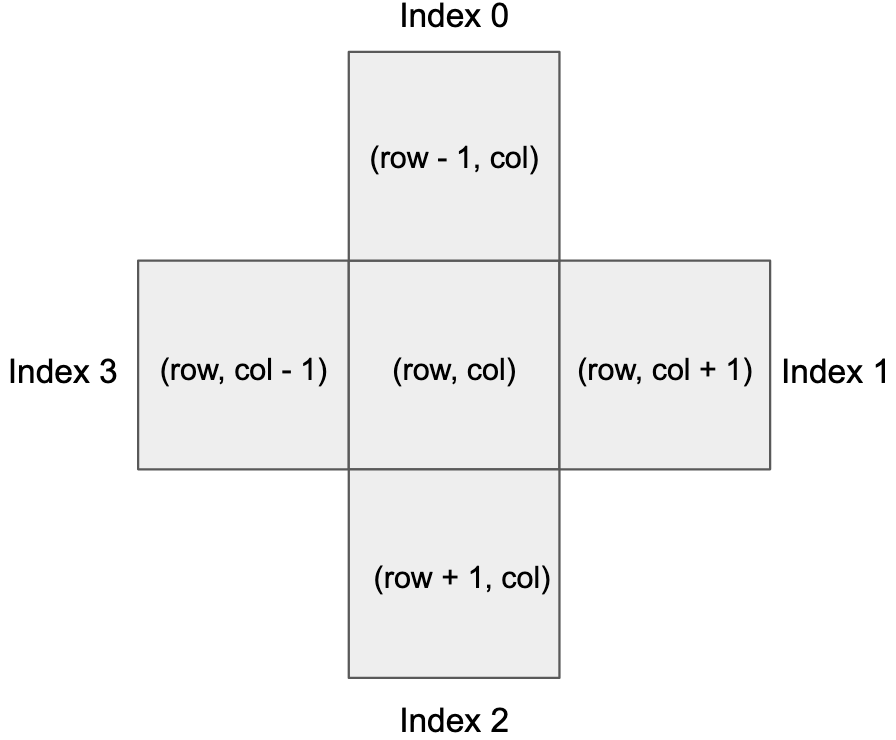
\includegraphics[scale=.45]{calculate_utility_diagram.png}
          % \caption{Example of a parametric plot ($\sin (x), \cos(x), x$)}
        \end{figure}
        \begin{table}[h!]
          \begin{center}
            \begin{tabular}{c|c|c}
              \textbf{Intended Action} & \textbf{90$^{\circ}$ Anti-Clockwise Action} & \textbf{90$^{\circ}$ Clockwise Action}\\
              \hline
              North (index 0) & West (index 3) & East (index 1)\\
              East (index 1) & North (index 0) & South (index 2)\\
              South (index 2) & East (index 1) & West (index 3)\\
              West (index 3) & South (index 2) & North (index 0)\\
            \end{tabular}
            \caption{Possible actions undertaken due to probability depending on intended action.}
            \label{tab:table1}
          \end{center}
        \end{table}
        Then, multiply the coordinate's utility/reward value by the corresponding probability.



  \section*{Performance Analysis}


  \section*{Conclusion}
  none

\end{document}

% As  you  work  through  your  implementation  of  the  MDP-solver,  you  will  find  that  you  are  makinglots  of  decisions  about  how  precisely  to  translate  your  ideas  into  working  code.  The  report  should explain  these  at  length.
% The  perfect  report  will  give  enough  detail  that  we  don’t  feel  we  have  to read your code in order to understand what you code does (we will read it anyway).Given  the  requirement  for  your  code  to  be  based  around  an  MDP-solver,  you  would  be  wise  to include a description of how your code solves the MDP, and which bits of the code do this solving.
 % Make sure you highlight these aspects of your work, especially things that make your work unique.
% Your  report  should  also  analyse  the  performance  of  your  code.  Because  there  is  a  certain  amountof  randomness  in  the  behaviour  of  the  ghosts,  a  good  analysis  will  run  multiple  games  to  assessPacman’s performance.  For example, you might like to try running:python pacman.py -n 50 -q -p MDPAgent -l mediumClassicto get a statistically significant number of runs so that you can, for example, establish the averagescore with some accuracy.  (Of course, to decide whether this was a statistically significant number of runs,  you  would  have  to  do  some  statistical  analysis  —  it  might  well  need  more  runs.)  All  the conclusions that you present in your analysis should be justified by the data that you have collected
